\section{Program Breakdown}

\subsection{Introduction}
The program is written in java, providing a GUI interface to rapidly enable a wide variety of testing conditions. 

\subsection{MainThread}

The MainThread class is what really makes this application tick. As the name suggest the 
class provides a thread on which the simulation is ran on. This class is responsible for 
multiple things, mainly the initialization of the simulation, and the running of the 
simulation. First off, is creating all the sensors. The number of sensors, as well as the 
number of sectors, and range is determined by parameters from the GUI, modified by the 
sliders. Creating sensors can be further broken down into three steps;  deciding their 
placement, identifying the neighbours, and assigning each sensor to an algorithm. 
	
\subsection{Sensor Placement}

Sensor placement is not to a random position, as this can cause two problems. Sensors can be 
to far away to connect, or so close that they sit almost on top of each other. This was solved 
by determining valid placements for new sensors upon the placement of a sensor, with the first 
sensor place in the centre of the simulation space. After placing the first sensor, a random 
number generator determines (between 3 and 8) how many sensors can be place around the 
starting sensor. At a random angle, the first valid position is recorded at 90\% the sensor 
range, and then the remaining placements are placed equal-radian apart, surrounding the first 
sensor. Placement data also contains the position of the sensor that spawned the placement. 
This is used to help generate new sensors growing outwards. After the initial sensor 
placement, a valid placement is randomly chosen out of the valid placement list, and a new 
sensor is placed. For these new sensors, they generate new valid placements, but with a small 
difference. They generate between 2 and 5 sensors, which are spread out along a 180 arc, which 
is centred on the new sensor, faces away from the sensor that generated the new sensor. This 
style of placement generates graphs that are always connected, but that also grow in random 
directions. It makes it less likely for sensors to overlap, but when generating over 100 
sensors, overlaps begin to occur quite frequently.

\begin{figure}
\centering
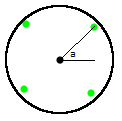
\includegraphics[height = 5cm]{pics/placement1.png}\\[0.5cm]    
\caption{Sensor Placement Example 1}
\floatfoot{The first sensor has been placed in the centre with placements shown in green. Between 3 and 8 sensors can be chosen to be placed (choose 4), first first at the random angle 'a'. The rest are placed equal-radian apart.}
\end{figure}

\begin{figure}
\centering
\caption{Sensor Placement Example 2}
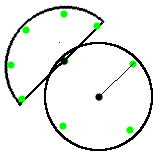
\includegraphics[height = 5cm]{pics/placement2.png}\\[0.5cm]  
\floatfoot{One of the placements was chosen to place a sensor, and is now black. A 180 degree semi-circle, facing away from the sensor that spawned the sensor we just placed (in this case, the original sensor). Between 2 and 5 sensor may be chosen as placements, this time 5. They are place equally distributed along the half circle, as seen with the new green circles. The next sensor can be any green circle, until all sensor are generated.}  
\end{figure}

\subsection{Neighbour Identification}

Two sensors are identified as neighbours if both are in range of each other, falling on some 
sector of each other. Neighbours are identified in the 'record\_neighbours' method in the 
MainThread. This method takes at most O(n2) times, since it runs on n sensors, checking at 
most, n other sensors. Each call to this method passes in the index of a sensor which needs to 
have it's neighbours identified. The method then loops through all the sensors up until the 
index passed in (all the sensors previously initialized). At each iteration of this loop, it 
checks if the sensor at the current iteration of the loop is in range of the sensor at the 
passed in index. If they are in range of each other, they are made neighbours and a prime 
number is determined from the 168 possible prime numbers for the sensor at the passed in 
index, such that no neighbourly sensors have the same prime number, thus effectively colouring 
the graph of sensors both graph theory-wise and literally the sensor's beam colour. 

\subsection{Assigning Algorithms}

After the neighbours are determined, each sensor is assigned to an algorithm, this taking O(n) 
time, as it goes through each sensor and assigns it to an algorithm. The type of algorithm 
that all the sensors will be assigned to is determined by a parameter from the GUI. After the 
initialization the MainThread is prepared to run.  The run method of the MainThread, runs 
until the application is stopped, either by completion, or the user clicking 'Stop'. It either 
re-initializes the sensors if the user has pressed 'New', or continues to run or re-run the 
simulation if the user clicks 'Start'. The main functionality that the run method provides is 
calling on update. In update, the algorithms are updated, taking an O(n), where n is the 
amount of algorithms that have not yet been complete. When a sensor is updated, it tells all 
the neighbour it is facing that it is no longer facing them, it increments to the next sector, 
and tells it's new neighbours that it is facing them. A neighbour is connected whenever both 
sensors it is linked to are 'facing'. Sensors stop checking neighbours that have been 
connected, speeding up their update time. An algorithm is complete when there are no remaining 
neighbours for it's sensor that need to be connected. Once the algorithm is complete it is 
then removed from the list. This is to done to significantly improve the overall performance 
of the application, since the purpose of the simulation is to demonstrate how sensors discover 
each other, once a sensor has discovered all of it's neighbourly sensors there is no need for 
it to keep searching/being updated. After the update has happened on the algorithms, the 
neighbours are checked for connection, followed by output to both the GUI and log, and a call 
to re-draw the sensors on the GUI. 
	
\begin{figure}
\centering
\caption{UML Diagram}
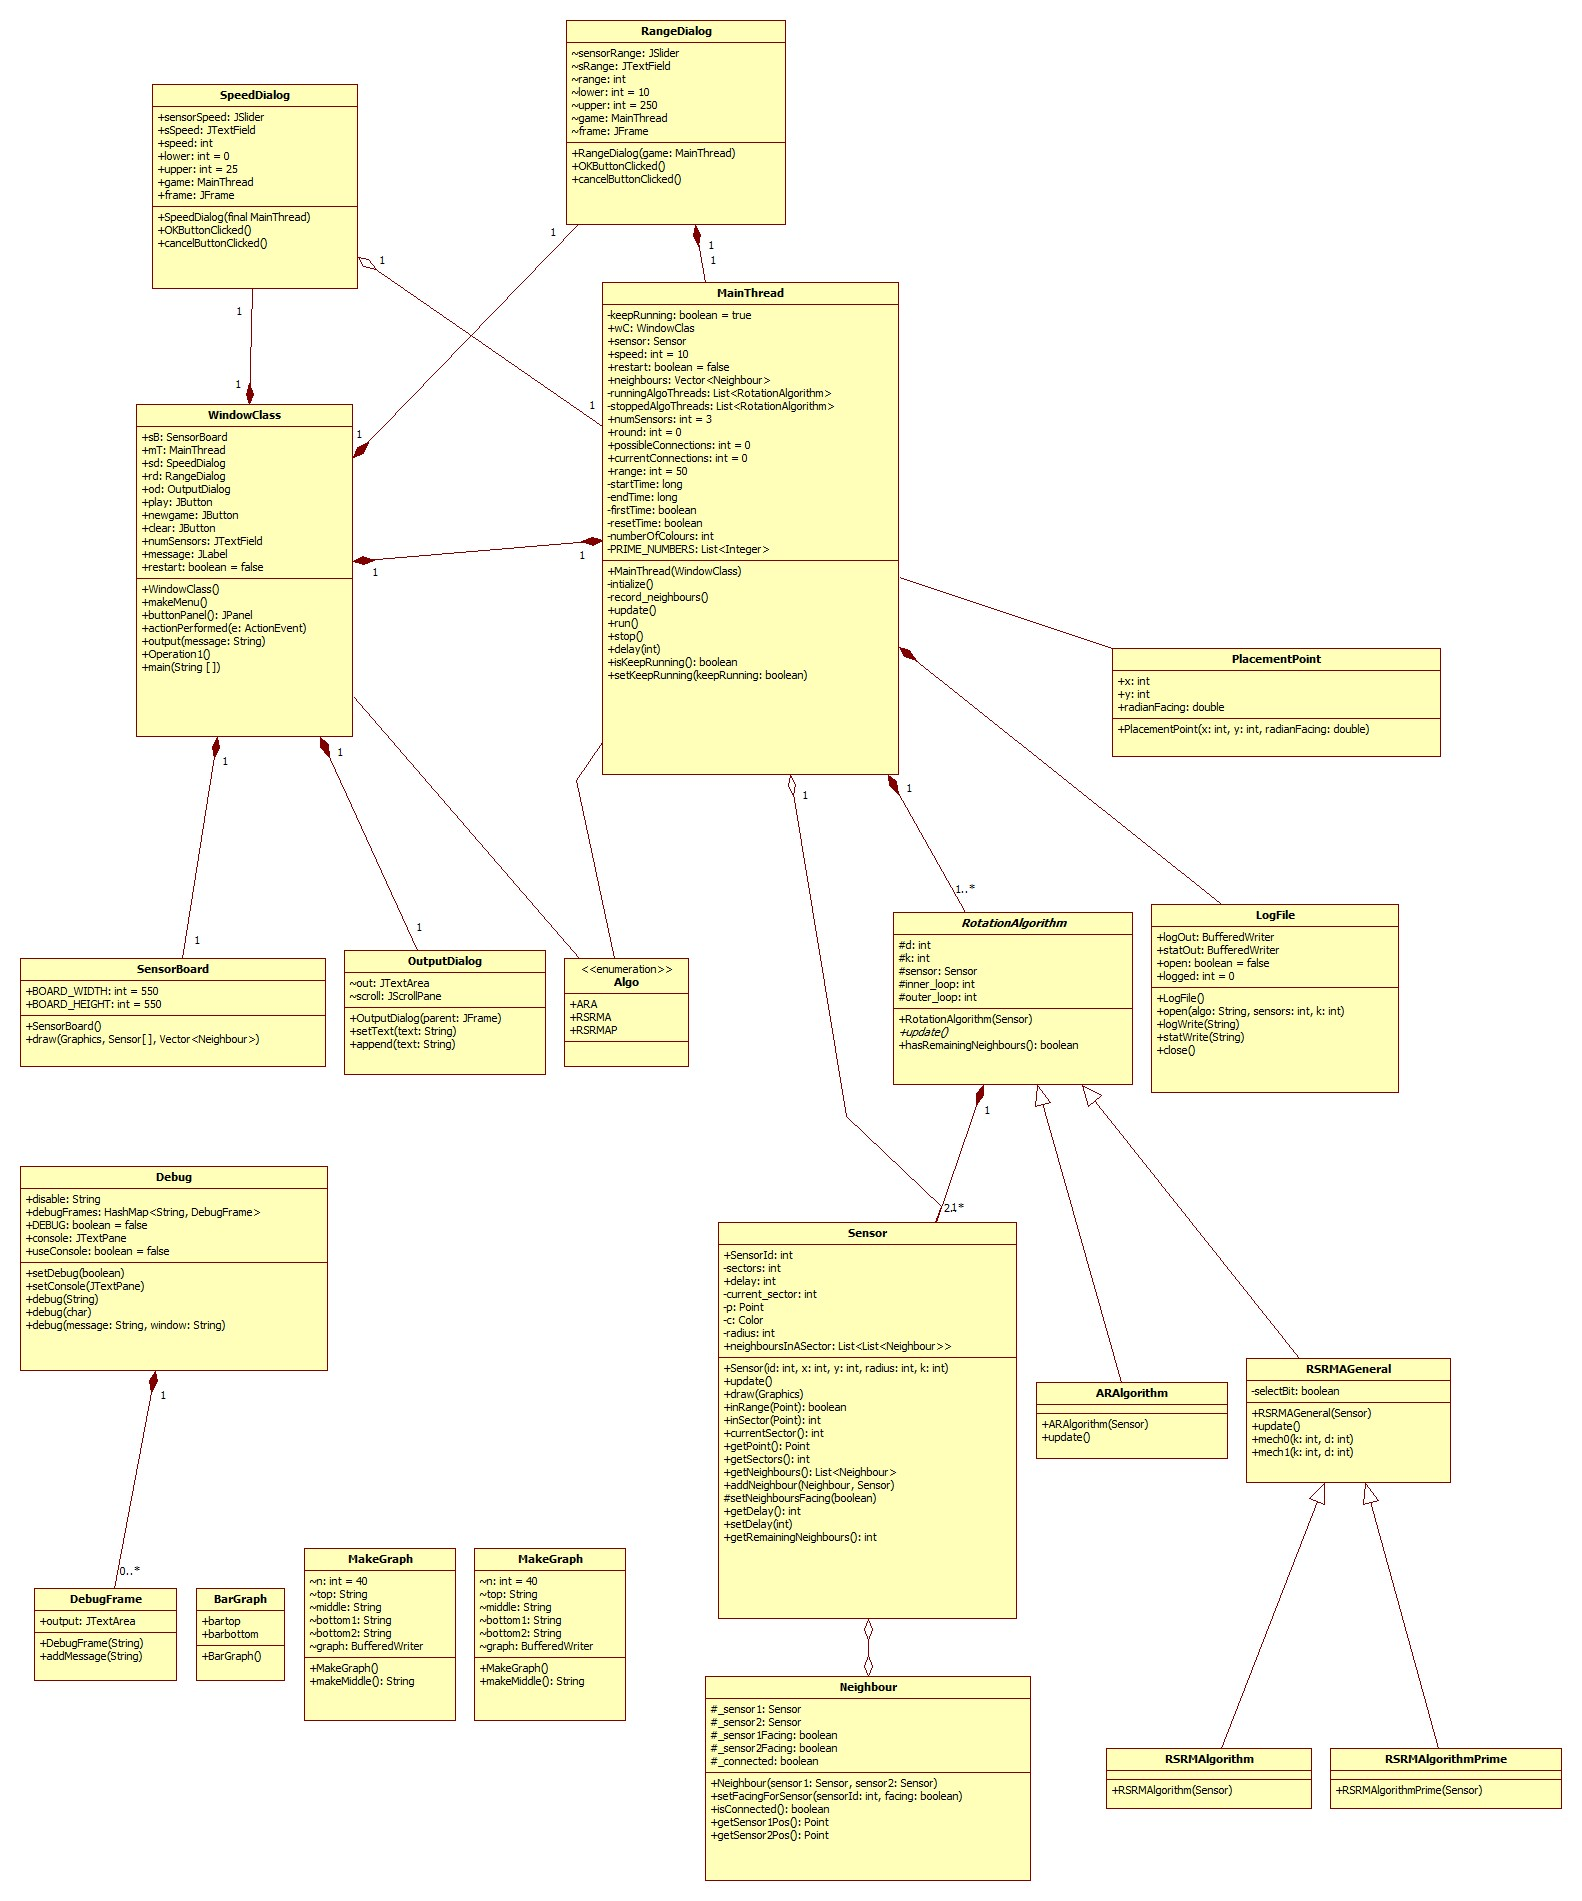
\includegraphics[height = 20cm]{pics/Main.jpg}\\[0.5cm]    
\end{figure}

\subsection{Running the Simulation}

The current approach MainThread takes for "running" the sensors, is that there is a list of 
algorithms that are each responsible for "running" their sensors. The algorithms themselves 
are all updating in the update method of the MainThread, and the MainThread is the only class 
responsible for spawning one thread that then repeatedly calls on update. The other approach 
would have been to allow each individual algorithm to spawn their own threads, which would 
then "run"/update the sensors, while the MainThread handles checking neighbour connects and 
calling on the GUI re-draw. During the development of this application, we had implemented 
this method. We've found that allowing each algorithm to have it's own separate thread could 
cause synchronization problems, but would model a more practical simulation. However, having 
just one thread for MainThread and repeatedly updating the algorithms in the update method, 
the way that the runs application now, models a more theoretical simulation where everything 
is updated synchronously, and thus this way was chosen to better demonstrate how the 
algorithms function and how the sensors discover each other.


\subsection{Rotation Algorithms}

\begin{figure}[ht]
\centering
\caption{Rotation Algorithms UML}
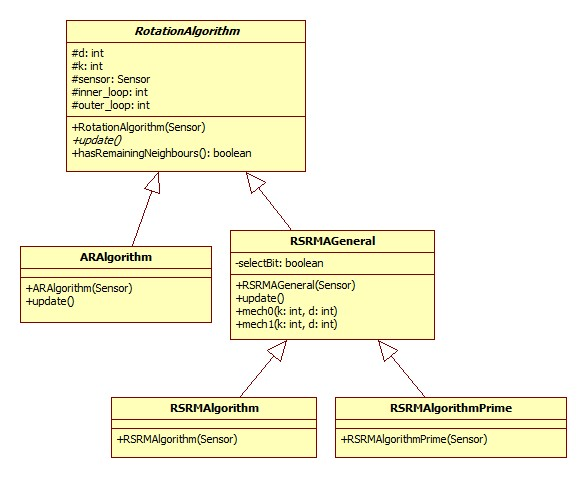
\includegraphics[height = 8cm]{pics/algo.jpg}\\[0.5cm]    
\label{fig:rotalgo}
\end{figure}

To implement the rotation algorithms we have decided to use a strategy pattern, as shown in 
Figure \ref{fig:rotalgo}, to allow the MainThread to update a RotationAlgorithm without 
specifically knowing which type it is. The main thread includes a List of RotationAlgorithms 
that get initialized, based on GUI parameters, to a more specific algorithm such as ARA, 
RSRMA, or RSRMA' . It was easy to see that a strategy pattern was needed, simply because all 
the algorithms shared a number of things in common. Using the strategy pattern allowed us to 
abstract common methods and variables, such as the delay (d), sectors (k) variables and mech0 
and mech1 methods. This produced more elegant code. Each algorithm takes in a Sensor that it 
will be responsible for rotating, and based on that sensor, it determines the algorithm's 
delay (d) and number of sectors (k).  Because these algorithms do not spawn their own threads 
and rely on the MainThread to loop through them, the delay loops were done slightly 
differently. The update method for each algorithm is responsible for rotating the Sensor. In 
the update methods the outer\_loop and inner\_loop variables are used to simulate delay. In the 
case of the ARAlgorithm, where the original algorithm is described in the assignment and the 
additional papers, the for-loop inside of the while-loop acted as a delay. It was implemented 
so that the while-loop was the MainThread update loop and the inner for-loop was represented 
by the outer\_loop variable, to cause delay. To be more specific, the outer\_loop variable upon 
initialization of an ARAlgorithm is set to the sensor's 'd', it's color/prime. Every time the 
update happens for the ARAlgorithm, the outer\_loop variable decrements, until it reaches zero. 
When it is zero the sensor updates, causing a turn, and the outer\_loop variable is re-
initiated to the sensor's 'd'. This simulates the delay in the algorithm, and although the 
loop does not look the same, it functions the same way. For the RSRMA and RSRMA' the loops 
were handled in a similar fashion. However each time the outer\_loop variable reached zero, it 
would randomly pick between mech0 and mech1. With the level of abstraction that was made by 
implementing the strategy pattern, the RSRMAGeneral contained the majority of how the 
randomized algorithms functioned. It was noticed that the difference between RSRMA and RSRMA' 
was that one passed in two 'k', treating one of the 'k's as a 'd', while the other passed in 
'k' and 'd' to the mechs. Thus the only code that RSRMAlgorithm and RSRMAlgorithmPrime possess 
is their constructors, where the former assigns the Sensor's 'k' value to its 'k' and 'd', and 
the later assigns its Sensor's 'k' and 'd' values to it's own 'k' and 'd' values, 
respectively.


\subsection{GUI Interface}
The GUI has some configurable sections. In particular there are slider settings for running speed, the number of sectors and the range. We are technically running the tests in a unit square, so the range has no applicative meaning except in the sense of the visual output (ie it makes bigger circles on screen), but it will also have an impact on graph density (ie higher range values, as a fraction of the unit square, will mean more connections and a denser graph). The selection of the colouring of the sensor beams is based on the "colouring" of the graph, so that sensors that have the same colouring (ie prime number delay) will be dislayed with the same colour onscreen.

In addition there is a plain output window that shows the same text that is being output to the logfile, including the number of connections made and the number of connections left to be made. This allows you to monitor the state of the algorithm as it is running.

\subsection{Known Issues}
One issue is with our update loop. Because a sensor is moved and updates its connections in the same loop, it is possible to connect to a sensor that is scheduled to move later in the loop, where technically it shouldn't. In terms of performance it may mean a slightly better performance for every algorithm, but since every algorithm has the same potential advantage the overall comparison is not affected. This will occasionally manifest itself as the final sensors finishing out of alignment in the GUI. It does seem quite rare in practice however.
 